\chapter{提案手法}
\label{solv}

本章では、低遅延な広域Layer 2ネットワークを構築するにあたり想定する環境を整理した上で、本研究で
提案するシステムの概要について述べる。

\section{設計}

\begin{figure}
	\begin{center}
		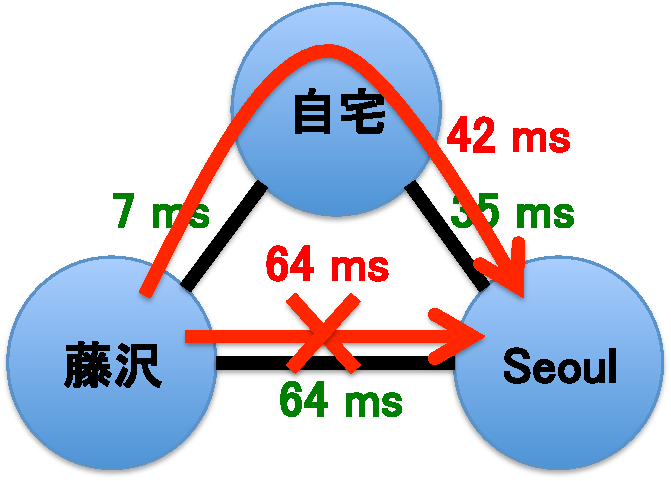
\includegraphics[scale=0.60]{./img/betterpath}
		\caption{他拠点を経由させることによる遅延の削減}
		\label{img:betterpath}
	\end{center}
\end{figure}

本研究では、まずトンネル終端点が、トンネル終端点間の遅延を計測し、その計測結果に基づいた経路選択が行えるようにする。
例えば、図~\ref{img:betterpath}で示すように、藤沢、自宅とソウルの3拠点に同一のLayer 2ネットワークを拡張するとする。この場合、
藤沢とソウルの間で通信するにあたり、インターネットの経路で直接転送するよりも、自宅を経由
することにより約35\%小さい遅延で通信することが可能である。Layer 2ネットワーク拡張技術は、このような経路を発見するために、
Layer 2ネットワークに参加している全トンネル終端点の遅延を計測する。そして、遅延が最も小さくなる経路を計測結果から計算し、その経路でイーサネットフレームの
転送を行う。

また、インターネット上で分散して動作するよう、トンネル終端点が個々でLayer 2ネットワークに参加しているトンネル終端点のリスト
を管理するようにする。トンネル終端点はLayer 2ネットワークへの参加や離脱などのメッセージを、Layer 2ネットワークに参加している
全てのトンネル終端点に広告する。これにより、全てのトンネル終端点でLayer 2ネットワークに参加しているトンネル終端点のリストを共有する。
また、全てのトンネル終端点に転送する必要があるイーサネットフレームは、SupernodeやIPマルチキャストに転送するのではなく、全てのトンネル終端点に1つ1つ転送する。
これにより、SupernodeやIPマルチキャストが不要となり、インターネット上で分散して動作するLayer 2ネットワークを構築することができる。


\section{想定環境}
\label{solv:env}

本研究の目的は、インターネット上でサービスを提供しているサービスプロバイダーが、
インターネット上に分散された複数の拠点に同一のLayer 2ネットワークを拡張する際に、拡張されたLayer 2ネットワーク上で
動作するサービスの遅延によるパフォーマンス低下を小さくすることである。
拠点の数は数十拠点を想定する。また、拠点の場所は国内、及び、その近隣諸国とする。インターネット上
に拠点が分散しているような環境では、現在のインターネットに存在する経路の問題に
より、宛先と直接通信するより、別の拠点を経由して宛先に到達するほうが
低遅延で通信できる場合がある。そこで本研究では、遅延を小さくするために、イーサネットフレームを転送する際に
遅延の最も小さい経路で転送をすることができるLayer 2ネットワーク拡張技術を提案する。これが実現することにより、従来の手法
と比べ、拡張されたLayer 2ネットワーク上で動作するアプリケーション
のパフォーマンスが向上されることが期待される。

本研究では拡張されたLayer 2ネットワーク上で利用されるアプリケーションとしてNFSv3を
想定する。複数の拠点に分散したサービスを構築するためには、同じデータを全拠点
からアクセスできることが必要となる場合がある。複数の拠点から共通のデータを利用する手段として
NFSv3を利用するという手法が挙げられる。しかし、NFSv3は遅延がとても小さい、単一の拠点内で運用され
るように設計されているため、遅延の大きい環境で利用した場合、パフォーマンスが著しく低下する。本研究では
このような低遅延を要求するアプリケーションを想定アプリケーションとする。

\section{機能要件}
\label{solv:requirements}

前節で説明したような環境で、低遅延な拡張されたLayer 2ネットワークを実現するための
Layer 2ネットワーク拡張技術に対する要件は以下の通りである。

\begin{itemize}
	\item{インターネット上に分散された複数の拠点へのLayer 2ネットワークの拡張}
	\item{宛先に応じた転送先の選択}
	\item{遅延の最も小さい経路でのイーサネットフレームの転送}
	\item{分散して動作すること}
\end{itemize}

低遅延な拡張されたLayer 2ネットワークを構築するためには、遅延の最も小さい経路でイーサネットフレームが転送
される必要がある。これを実現するために、まずLayer 2ネットワーク拡張技術は参加している全てのトンネル終端点間の
遅延を計測し、その計測結果を用いて遅延が最も小さい経路を計算する。そしてトンネル終端点が、
イーサネットフレームを転送する際には、イーサネットフレームの宛先に応じて転送するトンネル終端点を選択し、
計算した経路に基いて転送を行う。宛先の
トンネル終端点に直接転送する場合が最も遅延の小さい経路の場合には直接転送をする。他のトンネル終端点を経由して宛先
に転送したほうが小さい遅延で転送できる場合は、他のトンネル終端点を中継する。また、
インターネット上に分散された複数の拠点にLayer 2ネットワークを拡張することができる必要がある。
さらに、どこかの拠点で障害が発生した場合でも、正常にLayer 2ネットワークが動作していることが求められる。
そのため、Supernodeなどといった中心となるサーバーやIPマルチキャストが必要なく、分散して動作する必要がある。

\section{システム概要}
\label{solv:requiredl2}

\begin{figure}
	\begin{center}
		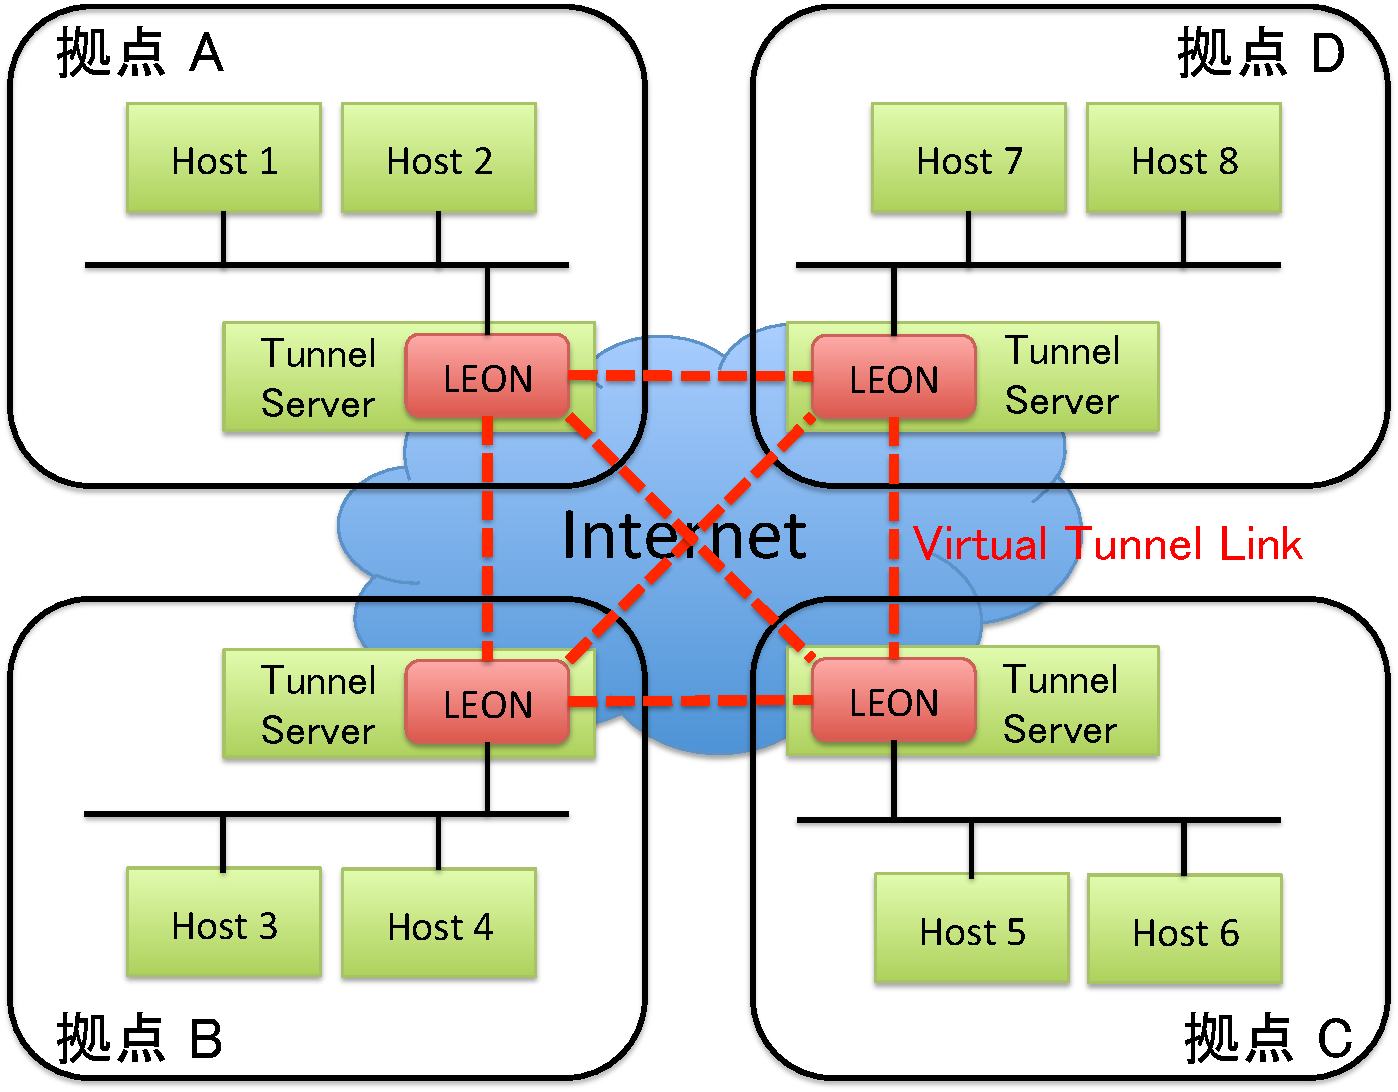
\includegraphics[scale=0.60]{./img/mtuntopology}
		\caption{LEONによって構築されるLayer 2ネットワークトポロジー}
		\label{img:mtuntopology}
	\end{center}
\end{figure}


本研究では、前節で示した機能要件を実現する低遅延Layer 2ネットワーク拡張手法として、
Latency Efficient Overlay Network (LEON)を提案する。LEONはIPネットワークを経由してイーサネットフレーム
を転送するLayer 2ネットワーク拡張技術である。LEONによって構築されるLayer 2ネットワーク
のトポロジーを図~\ref{img:mtuntopology}に示した。LEONを動かし、トンネル終端点として
動作するサーバーは各拠点に1つ設置する。トンネル終端点として動作するサーバーはインターネット
と拡張されたLayer 2ネットワークに所属するホストが収容されているLayer 2ネットワークに接続されている。
そして、LEONは自分の拠点に所属しているホストが、他拠点に設置されているホストと通信するための
ゲートウェイとして動作する。

\begin{figure}
	\begin{center}
		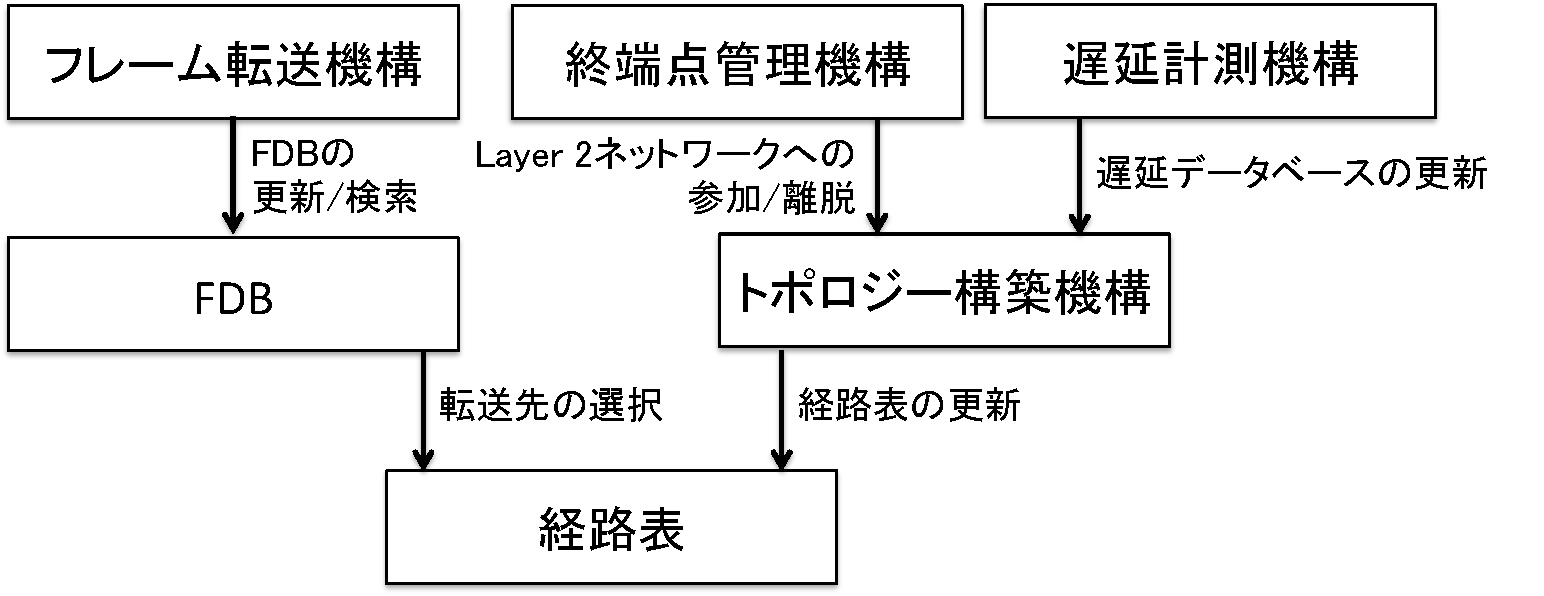
\includegraphics[scale=0.65]{./img/mtunworks}
		\caption{LEONのシステム概要}
		\label{img:mtuntopology}
	\end{center}
\end{figure}

LEONのシステム概要を図~\ref{img:mtuntopology}に示す。まず、LEONは既にLayer 2ネットワークに参加している
トンネル終端点を学習する。トンネル終端点の学習後、トンネル終端点間の遅延を計測する。トンネル終端点間の
遅延は時間帯に応じて変化する可能性があるため、トンネル終端点の学習時のみだけでなく、定期的に実行される。
また、遅延の計測結果は他トンネル終端点に広告する。そして、全てのトンネル終端点への遅延計測が完了後、
各トンネル終端点と通信する際に遅延が最も小さくなる経路を計算する。ここで計算された経路は経路表にする。
LEONが転送すべきイーサネットフレームを受信した際には、ホストがどのトンネル終端点に収容されているかが記録されている
データベースを参照し、イーサネットフレームの宛先ホストがどのトンネル終端点によって収容されているのか検索する。そして、
事前に計算された経路表に基づき、イーサネットフレームを宛先ホストが収容されているトンネル終端点へ転送する。

トンネル終端点の学習は、トンネル終端点を管理するサーバーなどを用いず、トンネル
終端点間で自律的に行う。トンネル終端点を管理するサーバーを用意することにより、Layer 2ネットワークに参加
しているトンネル終端点の学習やトンネル終端点間のメッセージングは容易となる。しかし、トンネル終端点を
管理するサーバーが単一障害点となってしまい、障害発生時には拡張されたLayer 2ネットワークの通信全体に
影響を与えてしまう可能性がある。トンネル終端点が自律的に他のトンネル終端点を学習できた場合、トンネル終端点
を管理するサーバーが必要なくなり、どれかのトンネル終端点で障害が発生したとしても、影響を受けるのは
障害が発生しているトンネル終端点だけである。そのため、LEONでは他トンネル終端点をトンネル終端点が
自律的に学習できるようにする。

\begin{figure}
	\begin{center}
		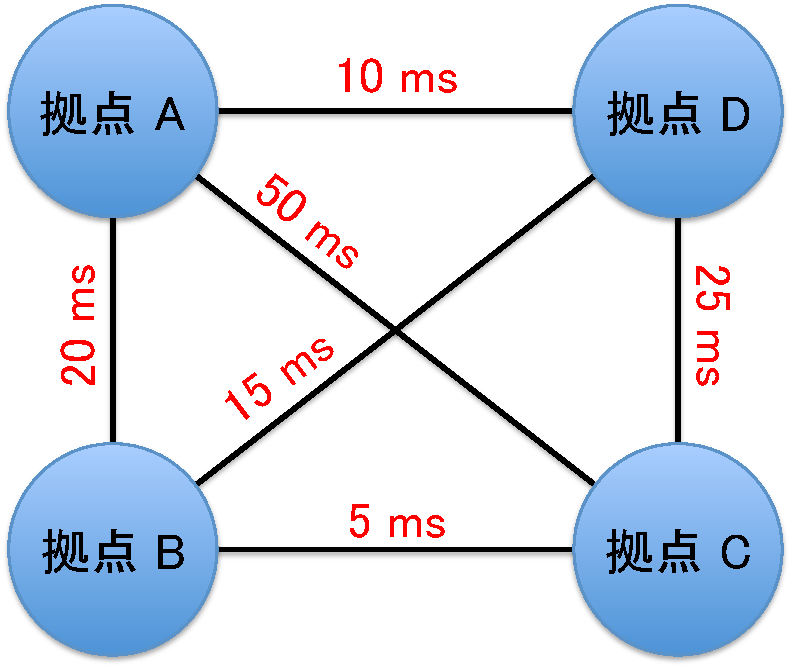
\includegraphics[scale=0.60]{./img/rttascost}
		\caption{RTTをコストとした経路の選択}
		\label{img:rttascost}
	\end{center}
\end{figure}

学習されたトンネル終端点へ到達するための経路は、トンネル終端点間の遅延に基いて選択する。
~\ref{background:internetroute}節で説明したように、現在のインターネット
の経路は宛先までの遅延やリンクの使用率などが考慮されていないため、遅延が最も小さい経路
でない場合がある。宛先にインターネットの経路で到達するよりも、他のトンネル終端点
を経由させたほうが遅延が小さくなる場合がある。そのため、遅延が最も小さい経路でイーサネットフレーム
を転送するためには、トンネル終端点は宛先のトンネル終端点に転送する際に、遅延が最も小さい経路
を計算する必要がある。LEONは、遅延が最も小さくなる経路を計算するために、トンネル終端点間
の遅延を計測する。また、計測された遅延の計測結果は、他のトンネル終端点が同様に計算するために
必要となるため、他のトンネル終端点にも広告する。収集された遅延の計測結果は、
図~\ref{img:rttascost}のようなトンネル終端点間の遅延関係を計算するために利用される。そして、
この遅延関係から遅延をコストとしたダイクストラ法~\cite{dijkstraalgo}を用いて、Layer 2ネットワーク
に参加している各トンネル終端点に到達するにあたり遅延が最も小さくなる経路を計算する。
宛先のトンネル終端点に到達するにあたり、インターネットの経路に基いて、直接転送する経路が
遅延が最も小さい経路であれば直接転送を行う。宛先のトンネル終端点に到達するにあたり、他の
トンネル終端点を経由する経路が遅延の最も小さい経路であれば、そのトンネル終端点に
中継してもらう。LEONでは、このような手法を用いて、Layer 2ネットワークに参加している
各トンネル終端点へ到達するための経路を選択する。

また、イーサネットフレームの転送は、前述した各トンネル終端点までの経路とは別に、どのホストが
どのトンネル終端点によって収容されているかを記録しているFowarding Database(=FDB)に
従って行われる。トンネル終端点は、イーサネットフレームを転送するにあたり、宛先ホストがどのトンネル
終端点によって収容されているのかという情報を事前に記録されている必要がある。LEONでは、ホスト
から送られてくるブロードキャストフレームから、自動的にFDBの更新を行う。他トンネル終端点
からブロードキャストフレームが送られてきた際には、ブロードキャストフレームの送信元MACアドレス
とそのイーサネットフレームを転送したトンネル終端点をFDBに記録する。既知の送信元MACアドレス
が、記録されているトンネル終端点とは違うトンネル終端点から
転送されてきた際には、FDBの更新を行う。そして、イーサネットフレームを送信する際には、
宛先ホストがどのトンネル終端点によって収容されているのかをFDBから検索し、その情報と
事前に計算を行った経路に基いて転送を行う。

\begin{figure}
	\begin{center}
		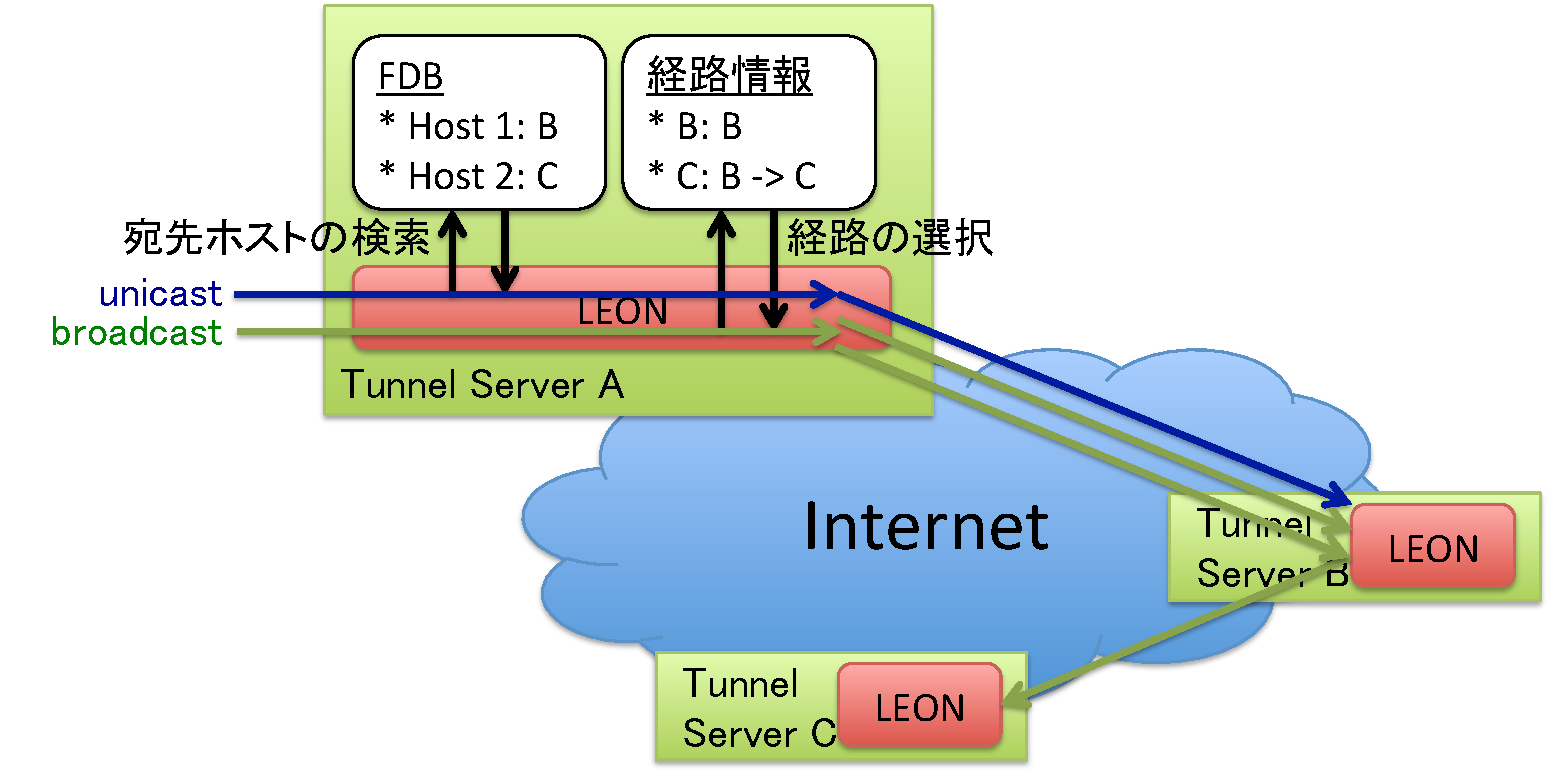
\includegraphics[scale=0.60]{./img/forwardabst}
		\caption{転送動作の概要}
		\label{img:forwardabst}
	\end{center}
\end{figure}

イーサネットフレームの転送は、各トンネル終端点がそれぞれ持つ経路表と自動的に学習された
FDBをもとに、宛先ホストまでの遅延が最も小さい経路で転送される。転送動作の概要を図~\ref{img:forwardabst}
に示す。トンネル終端点が転送
するイーサネットフレームを受け取ると、そのイーサネットフレームがユニキャストフレームか
ブロードキャストフレームかを判別する。ユニキャストフレームの場合、宛先ホストがどの
トンネル終端点によって収容されているかFDBから検索する。そして、経路表に従い、
宛先までの遅延が最も小さい経路で転送するための転送先を決定する。ブロードキャストフレームの場合は、
宛先ホストが所属しているトンネル終端点として全てのトンネル終端点を選択し、それぞれの
トンネル終端点に転送するにあたり、遅延が最も小さい経路で転送するための転送先を決定する。
インターネットの経路で宛先のトンネル終端点に到達することにより、遅延が最も小さく転送できるのであれば、転送先は宛先のトンネル終端点となる。
他のトンネル終端点を中継させることにより、遅延がインターネットの経路で直接転送した時よりも
小さくなるのであれば、転送先は中継するトンネル終端点となる。転送先が決定されると、
イーサネットフレームに転送経路が書かれたヘッダーと転送先のトンネル終端点が宛先となっているIPヘッダー
が追加され、インターネットにエンキャプシュレーションされたイーサネットフレームが転送される。
ユニキャストフレームの場合、転送先が1つなのでエンキャプシュレーション作業は1回のみである。
ブロードキャストフレームの場合、転送先が複数あるので、Layer 2ネットワークに参加しているトンネル終端点
の台数と同じ回数、エンキャプシュレーション作業が行われる。LEONではこのように、遅延が
最も小さい経路で、イーサネットフレームの転送を行う。

トンネル終端点が、エンキャプシュレーションされたイーサネットフレームを受信した際には、
イーサネットフレームに追加されたLEONヘッダーに記述された経路に応じて転送を行う。Layer 2ネットワーク上の
ホストから、他のトンネル終端点によって収容されているホストが宛先であるイーサネットフレームを受信した
トンネル終端点は、そのイーサネットフレームを転送する際に経路表から転送する経路を選択する。選択された経路は、
イーサネットフレームを転送する際に、イーサネットフレームの先頭に追加されるLEONヘッダーに記述される。
そして、トンネル終端点はエンキャプシュレーションされたイーサネットフレームを受け取ると、LEONヘッダー
に記述された経路を確認する。そのトンネル終端点が記述された経路の最後に書かれたトンネル終端点の場合は、その
トンネル終端点宛のイーサネットフレームであると判断し、送信元トンネル終端点によって追加されたIPヘッダー
とLEONヘッダーを取り外し、Layer 2ネットワーク上の宛先ホストへ転送をする。そのトンネル終端点が経路表の最後に書かれた
トンネル終端点でない場合は、そのトンネル終端点の次に記述されているトンネル終端点へイーサネットフレームを
さらに転送する。これにより、トンネル終端点は受信したエンキャプシュレーションされたイーサネットフレームの
転送先を決定する。

これにより、LEONは遅延が最も小さい経路でイーサネットフレームが転送されるLayer 2ネットワークの構築を行う。LEONはLayer 2ネットワーク
に参加しているトンネル終端点間の遅延を計測し、計測結果に基づき、イーサネットフレームの転送先
を選択する。最も遅延が小さくなる経路が、インターネット上の経路に基づいて転送する経路の場合、
インターネット上の経路でイーサネットフレームが転送される。他のトンネル終端点を経由する経路が
遅延の最も小さい経路の場合、経由すべきトンネル終端点に転送される。転送する際に、LEONは
転送経路が記述されたLEONヘッダーをイーサネットフレームに追加する。そして、転送されてきた
イーサネットフレームを受信した際には、LEONヘッダーのイーサネットフレームを参照し、受信した
トンネル終端点が経路の最後に記述されたトンネル終端点の場合は、イーサネットフレームの宛先
ホストへイーサネットフレームを転送する。受信したトンネル終端点が経路の最後に記述されたトンネル
終端点でない場合は、次に記述されているトンネル終端点へ受信したイーサネットフレームを転送する。
これにより、LEONはイーサネットフレームをインターネット上で遅延が最も小さい経路で転送する。

\section{プロトコルの設計}
\label{solv:protocol}

LEONは、遅延が最も小さい経路でイーサネットフレームが転送されるLayer 2ネットワークの構築と利用、そしてトンネル終端点間の遅延を
計測するために大きく分けて3種類のプロトコルを利用する。まず1つ目として、Layer 2ネットワークの
構築を行う際に利用されるコントロールプロトコルである。トンネル終端点は、コントロール
プロトコルを利用して、Layer 2ネットワークへの参加と離脱を行う。2つ目として、イーサネットフレーム
の転送を行う際に利用される転送プロトコルが挙げられる。転送プロトコルを利用して、Layer 2ネットワーク上の
イーサネットフレームがトンネル終端点間でやり取りされる。そして、3つ目として、トンネル終端点間の遅延情報の収集
を行う際に利用される計測プロトコルが挙げられる。計測プロトコルを利用して、トンネル終端点間
の遅延の計測とその計測結果のトンネル終端点間での共有を行う。これらのプロトコルは、全てUDPを
用いる。LEONが用いるメッセージの共通ヘッダーフォーマットを図~\ref{img:mtunheader}に示す。

\begin{figure}[h]
	\begin{center}
		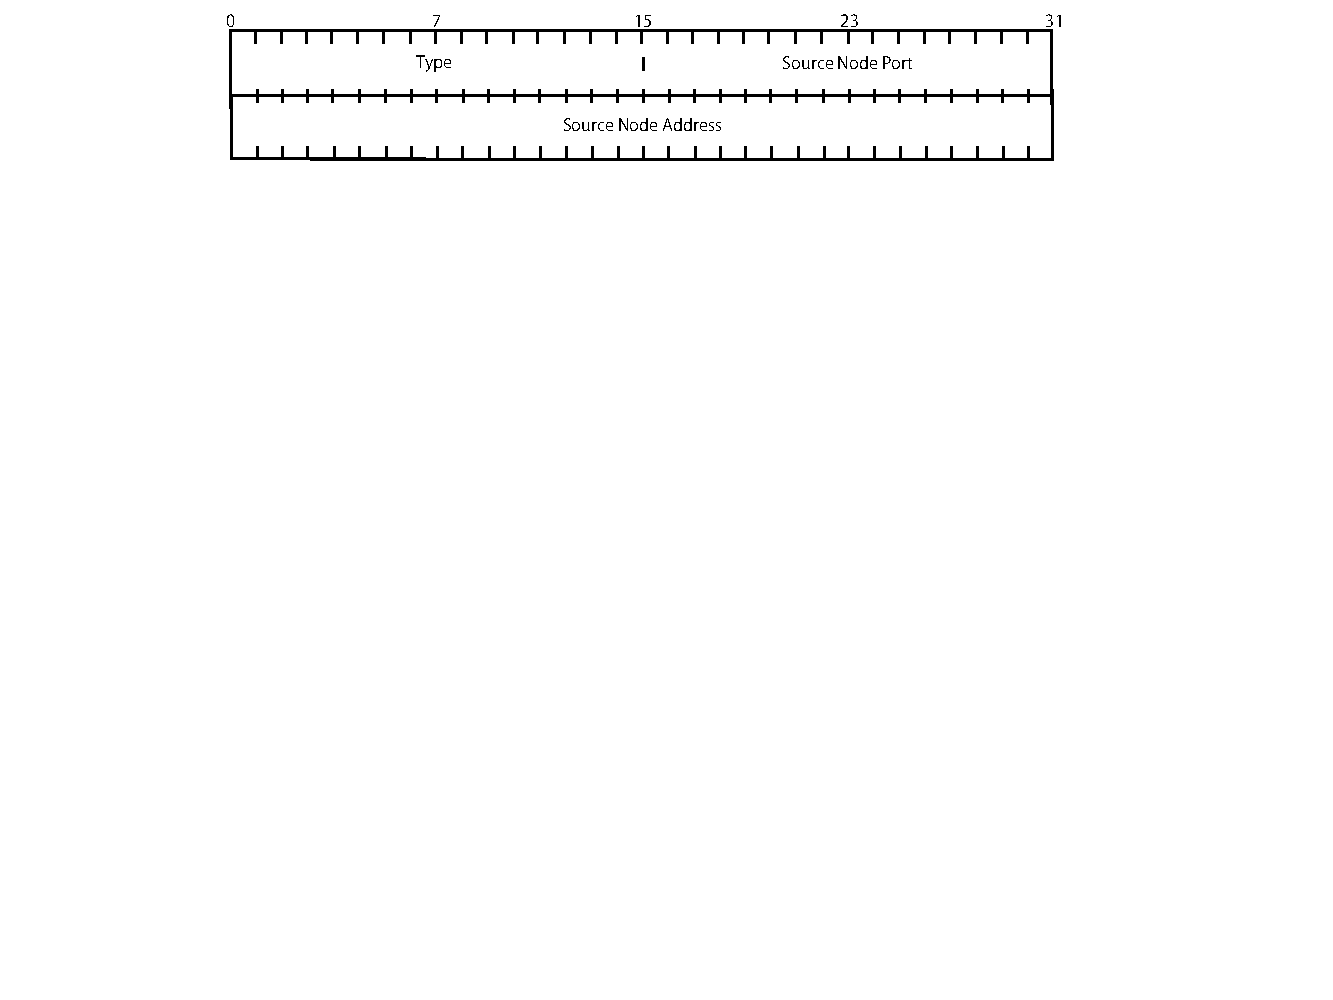
\includegraphics[scale=1.0]{./img/mtunheader}
		\caption{LEONの共通ヘッダーフォーマット}
		\label{img:mtunheader}
	\end{center}
\end{figure}

Typeフィールドは他トンネル終端点から送られてきたメッセージを識別するために利用される。
Typeの種類は全てで8種類である。まず、トンネル終端点がLayer 2ネットワークへ参加と離脱を行うための
コントロールプロトコルで利用されるTypeとしてJOINNODE(20)、JOINNODEACK(21)、DELNODE(30)、REQALL(40)の5種類
がある。次に、トンネル終端点間でイーサネットフレームの転送を行うための転送プロトコルで利用されるTypeとしてFORWARD(10)
の1種類がある。最後に、トンネル終端点間の遅延情報の収集を行うための遅延計測プロトコルで利用されるTypeとしてPINGREQ(50)、
PINGACK(51)、LATENCYDATA(60)の3種類がある。Source Node AddressとSource Node Portフィールドはメッセージの送信元トンネル終端点
のIPアドレスとポート番号が挿入されている。以下に、各プロトコルの詳細について述べる。

\subsection{コントロールプロトコル}
\label{solv:controlprotocol}

コントロールプロトコルはトンネル終端点がLayer 2ネットワークに参加と離脱を行う際に
用いられる。コントロールメッセージのフォーマットを図~\ref{img:controlheader}に示す。

\begin{figure}[h]
	\begin{center}
		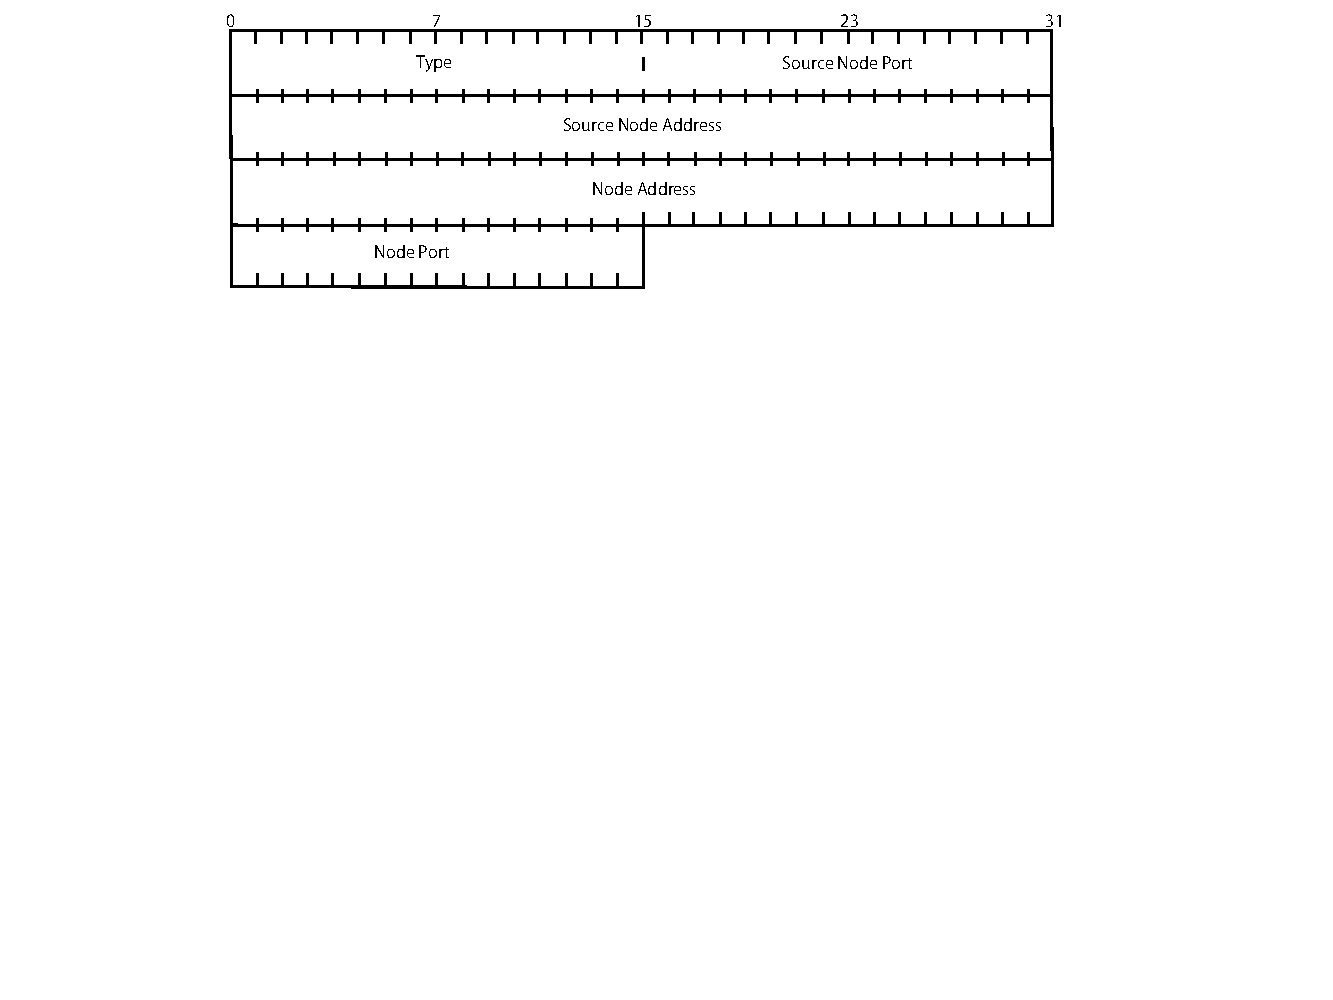
\includegraphics[scale=1.0]{./img/controlmessage}
		\caption{コントロールメッセージのフォーマット}
		\label{img:controlheader}
	\end{center}
\end{figure}

\begin{figure}
	\begin{center}
		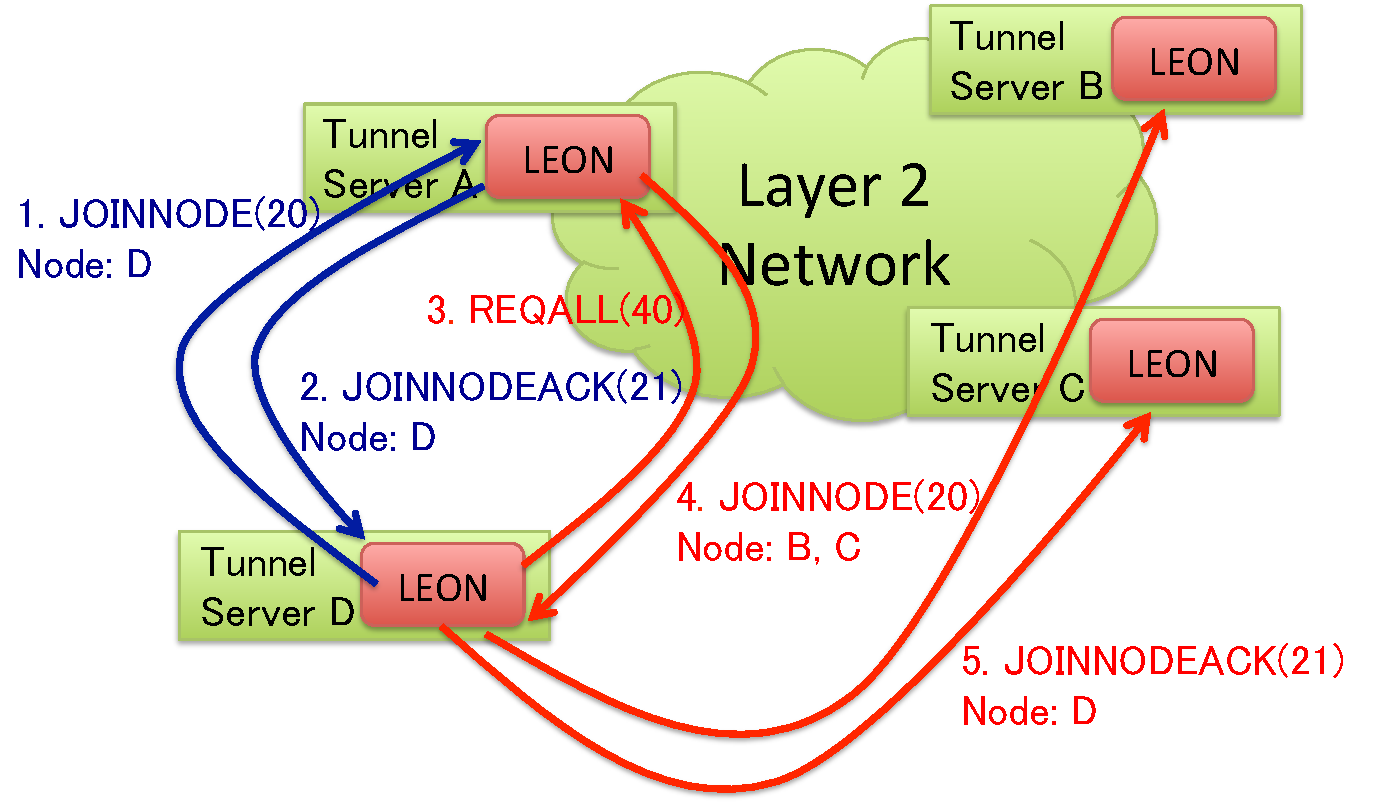
\includegraphics[scale=0.60]{./img/joinnodeproc}
		\caption{新規トンネル終端点の参加プロセス}
		\label{img:joinnodeproc}
	\end{center}
\end{figure}

トンネル終端点が新たに既存のLayer 2ネットワークに参加する際の手順を図~\ref{img:joinnodeproc}に示す。まず、既にLayer 2ネットワークに
参加しているトンネル終端点の1つにTypeフィールドがJOINNODE(20)であるコントロールメッセージを
送信する。このときコントロールメッセージのNode AddressフィールドとNode Portフィールドには、
新たに参加するトンネル終端点のIPアドレスとポート番号が挿入されている。送信された
コントロールメッセージを受信したトンネル終端点は、そのトンネル終端点が管理しているトンネル終端点
一覧に送信元トンネル終端点を追加する。そして、正常に受け取ったことを送信元トンネル終端点に通知するために、
JOINNODEACK(21)となっているコントロールメッセージを送信する。このときコントロールメッセージの
Node AddressフィールドとNode Portフィールドは新たに参加したトンネル終端点のIPアドレスと
ポート番号が挿入されている。新たに参加するトンネル終端点が、JOINNODEACK(21)となっている
コントロールメッセージを受信すると、新たに参加するトンネル終端点が管理するトンネル終端点
一覧に既にLayer 2ネットワークに参加しているトンネル終端点の1つが登録される。次に、新たに参加するトンネル終端点は、
他の既にLayer 2ネットワークに参加しているトンネル終端点に対しても同様な登録作業を行う
必要があるため、登録作業を済ませたトンネル終端点から既に参加している全トンネル終端点の一覧を
取得する。一覧を取得するためには、TypeフィールドがREQALL(40)であるコントロールメッセージ
を送信する。このときコントロールメッセージのNode AddressフィールドとNode Portフィールド
は0である。このコントロールメッセージを受信したトンネル終端点は、TypeフィールドがJOINNODE(20)であるコントロールメッセージ
を全トンネル終端点分送り返す。Node AddressフィールドとNode Portフィールドに既に参加している
各トンネル終端点を挿入し、コントロールメッセージを送信する。新たに参加するトンネル終端点が
このコントロールメッセージを受信すると、自身が管理するトンネル終端点一覧にNode Addressフィールドと
Node Portフィールドに書かれたトンネル終端点を登録する。そして、登録したトンネル終端点に対して、
TypeフィールドがJOINNODEACK(21)であるコントロールメッセージを送信する。これにより、相手のトンネル終端点に
相手が管理しているトンネル終端点一覧に、新たなトンネル終端点の登録をしてもらう。
この手順で新たなトンネル終端点は既存のLayer 2ネットワークに参加する。

\begin{figure}
	\begin{center}
		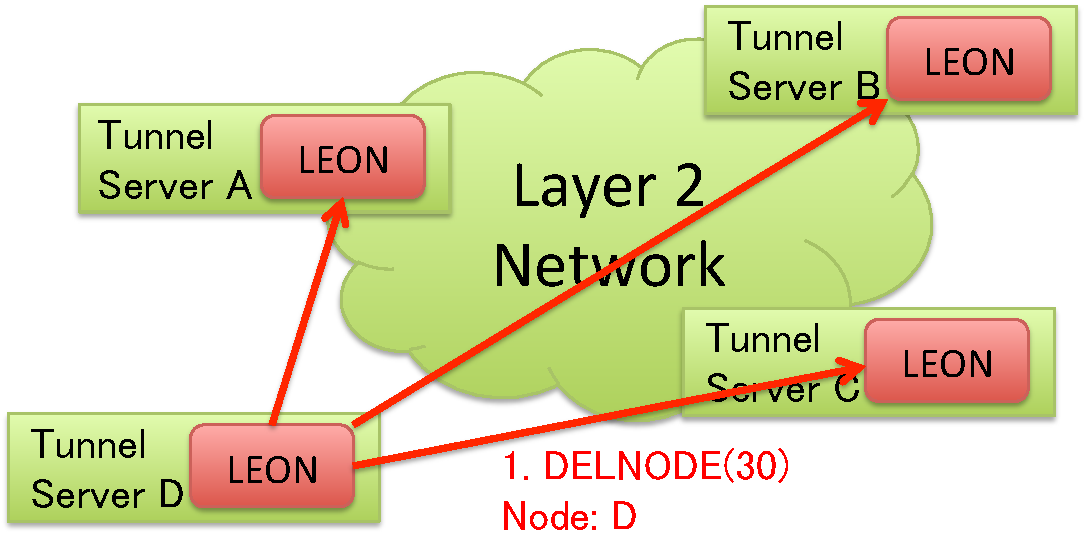
\includegraphics[scale=0.60]{./img/delnodeproc}
		\caption{トンネル終端点の離脱プロセス}
		\label{img:delnodeproc}
	\end{center}
\end{figure}

トンネル終端点が参加しているLayer 2ネットワークを離脱する際の手順を図~\ref{img:delnodeproc}に示す。
離脱するトンネル終端点は、トンネル終端点一覧に入っている
全てのトンネル終端点に対してTypeフィールドがDELNODE(30)であるコントロールメッセージを送信する。
このとき、Node AddressフィールドとNode Portフィールドには離脱するトンネル終端点のIPアドレスと
ポート番号が挿入される。そして、このコントロールメッセージを受信したトンネル終端点は、Node Address
フィールドとNode Portフィールドに挿入されたトンネル終端点をトンネル終端点一覧から削除する。
また、同時に、そのトンネル終端点によって収容されていたホストをFDBから削除する。これにより、
トンネル終端点は参加しているLayer 2ネットワークから離脱される。

\subsection{転送プロトコル}
\label{solv:fowardprotocol}

転送プロトコルはトンネル終端点が受信したイーサネットフレームを転送する際と、トンネル終端点が
イーサネットフレームを中継する際に用いられる。転送メッセージのフォーマットを図~\ref{img:forwardheader}
に示す。

\begin{figure}[h]
	\begin{center}
		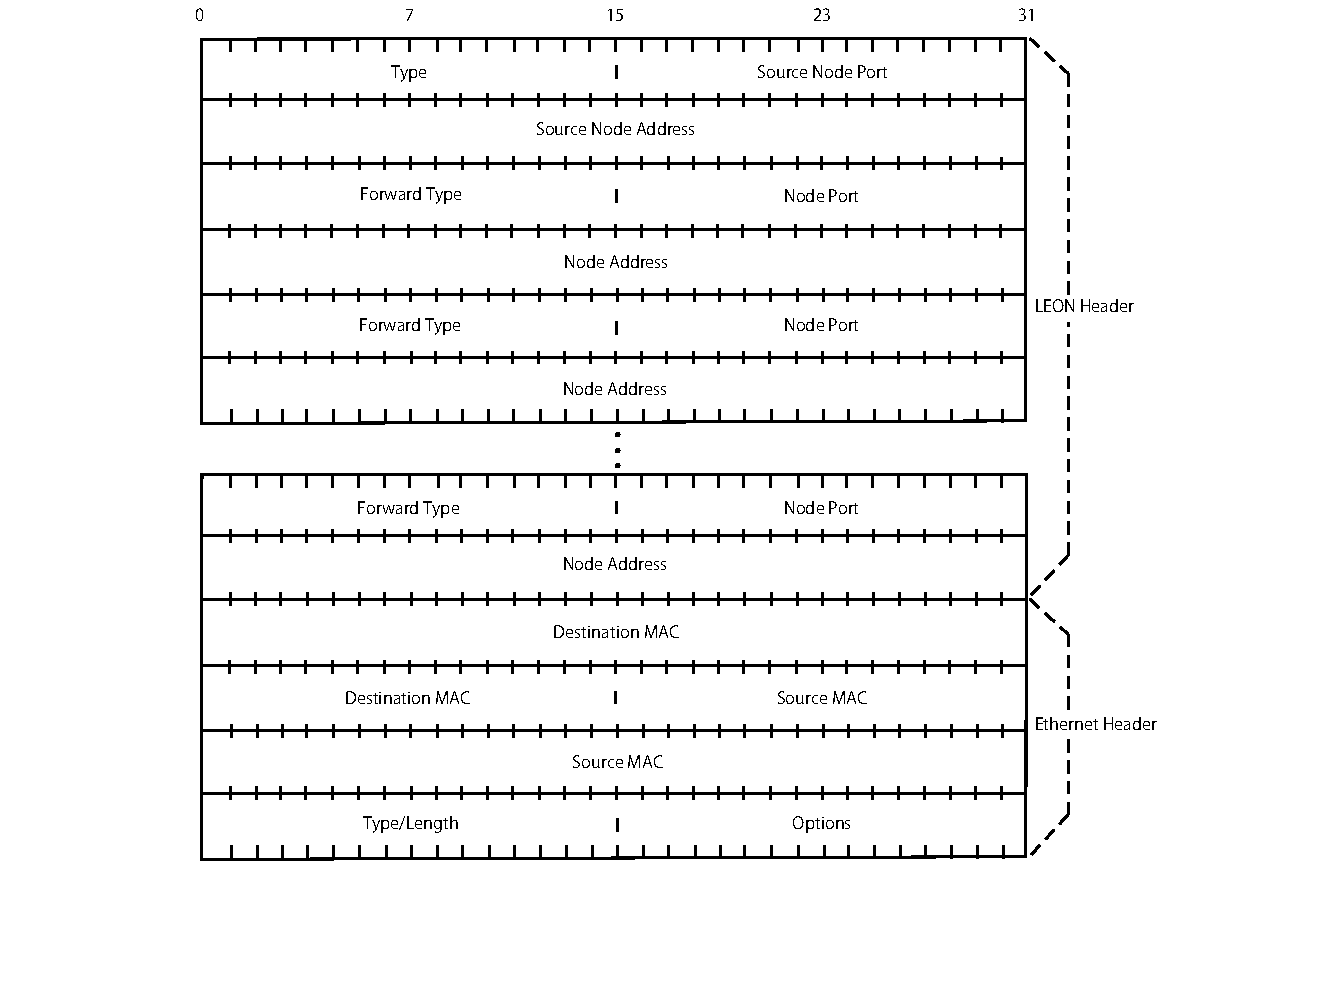
\includegraphics[scale=1.0]{./img/forwardheader}
		\caption{転送メッセージのパケットフォーマット}
		\label{img:forwardheader}
	\end{center}
\end{figure}

転送メッセージはLEONヘッダーとホストから受信したイーサネットフレームによって構成される。LEONヘッダーは
共通ヘッダーと転送経路情報で成り立っている。転送経路情報は転送メッセージを中継するトンネル終端点と
最終的に受信するトンネル終端点のリストである。トンネル終端点は転送メッセージをLEONヘッダーの転送経路情報
に従って転送する。転送メッセージのForward Typeフィールドは、次に書かれたトンネル終端点が中継するための
トンネル終端点か受信するトンネル終端点かを識別するためのものである。Foward TypeフィールドにはFORWARD(1)
またはRECEIVE(0)のどちらかを挿入する。そして、その次のNode Address及びNode Portフィールドには中継、または、
受信をするトンネル終端点のIPアドレスとポート番号を挿入する。転送経路情報の後ろにはホストから受信したイーサネット
フレームを付加する。

\begin{figure}
	\begin{center}
		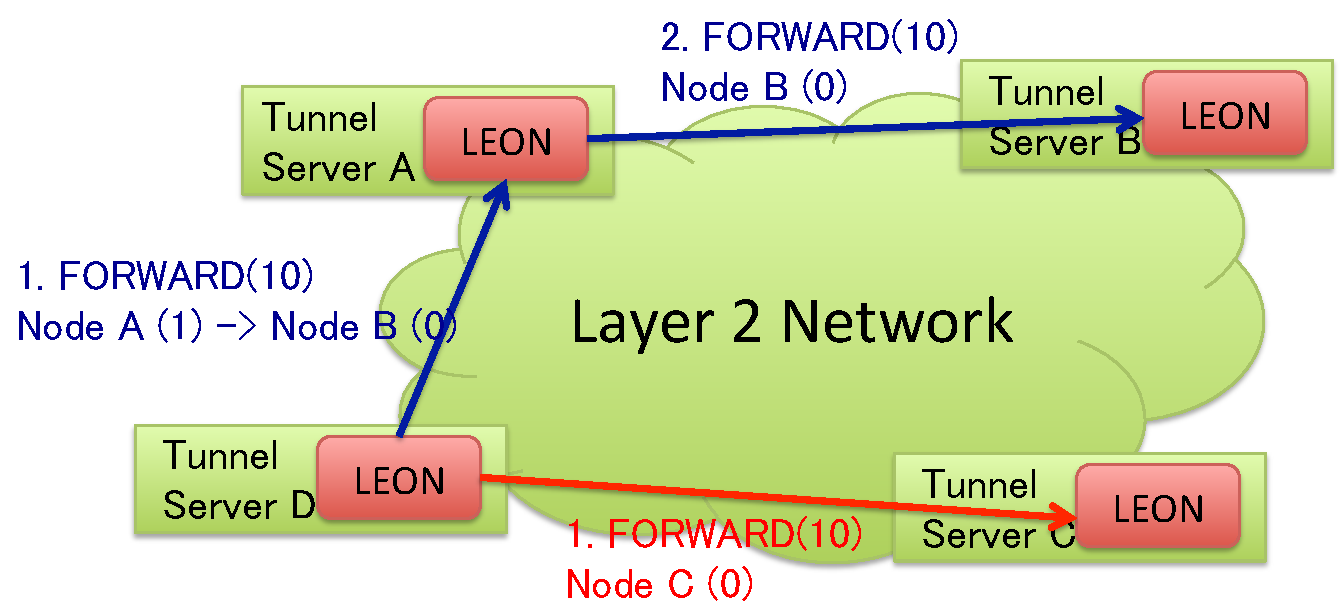
\includegraphics[scale=0.60]{./img/forwardproc}
		\caption{イーサネットフレームの転送プロセス}
		\label{img:fwdproc}
	\end{center}
\end{figure}

トンネル終端点が受信したイーサネットフレームを転送する際の手順を図~\ref{img:fwdproc}に示す。
トンネル終端点が収容しているホストからイーサネットフレームを受信すると、イーサネットフレームの
Destination MACフィールドを参照し、宛先のホストがどのトンネル終端点によって収容されているかFDB
から検索し、そのトンネル終端点までの経路を選択する。そして、イーサネットフレームの先頭にLEONヘッダー
を追加する。この際の共通ヘッダーのTypeフィールドはFORWARD(10)、Source Node AddressフィールドとSource Node Portフィールドは
イーサネットフレームを受信したトンネル終端点のIPアドレスとポート番号である。また、転送経路情報
の部分には選択された経路が挿入される。イーサネットフレームを直接宛先のトンネル終端点に転送する
場合は、転送経路情報はForward TypeフィールドがRECEIVE(0)、Node AddressフィールドとNode Portフィールドが宛先
トンネル終端点のIPアドレスとポート番号の1つである。イーサネットフレームを他のトンネル終端点を
中継して転送する場合は、転送経路情報はForward TypeフィールドがFORWARD(1)、Node Addressフィールドと
Node Portフィールドあ中継するトンネル終端点のIPアドレスとポート番号のヘッダー部分が中継するトンネル終端点
分追加される。そして、その後に最終的に受信するトンネル終端点のヘッダー部分を追加する。このとき追加される
ヘッダー部分は直接転送する場合のヘッダー部分と同じである。最後に、イーサネットフレームが
LEONヘッダーの後ろに追加される。

トンネル終端点が転送メッセージを受信すると自分を転送経路情報から探し、Forward Typeフィールドを
確認する。Forward TypeフィールドがRECEIVE(0)の場合、受信したトンネル終端点が最終的な宛先である
ことがわかる。トンネル終端点はLEONヘッダーを受信したパケットから取り除き、イーサネットフレーム
をLayer 2ネットワーク上の宛先ホストへ転送する。Foward TypeフィールドがFORWARD(1)の場合、受信した
トンネル終端点は中継用のトンネル終端点であることがわかる。トンネル終端点はLEONヘッダーの転送経路情報
から、そのトンネル終端点を転送経路情報からを消去し、次に指定されているトンネル終端点へ転送する。この際、最終的な宛先であるトンネル終端点が
、それがどのトンネル終端点から送信されたものか判別できるよう、共通ヘッダーのSource Node
AddressフィールドとSource Node Portフィールドの変更は行わない。

\subsection{遅延計測プロトコル}
\label{solv:latencyprotocol}

遅延計測プロトコルはトンネル終端点間の遅延の計測と、その計測結果の共有に用いられる。遅延の計測を行うための
遅延計測メッセージのフォーマットを図~\ref{img:ldcmessage}に示す。また、計測結果を共有するための遅延データ
メッセージのフォーマットを図~\ref{img:ldmessage}に示す。


\begin{figure}[h]
	\begin{center}
		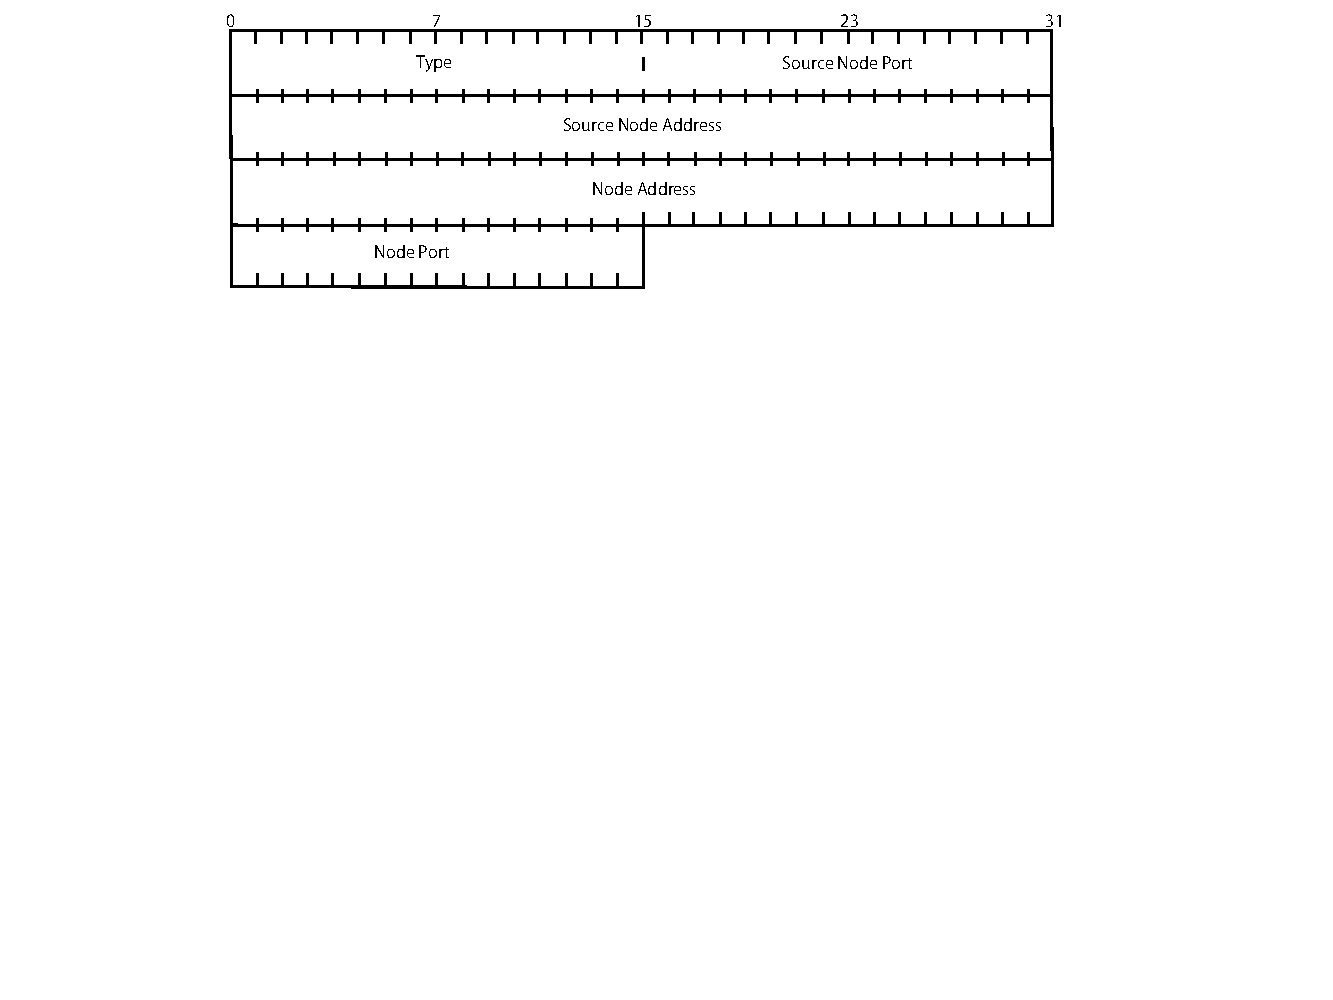
\includegraphics[scale=1.0]{./img/controlmessage}
		\caption{遅延計測メッセージのフォーマット}
		\label{img:ldcmessage}
	\end{center}
\end{figure}

\begin{figure}[h]
	\begin{center}
		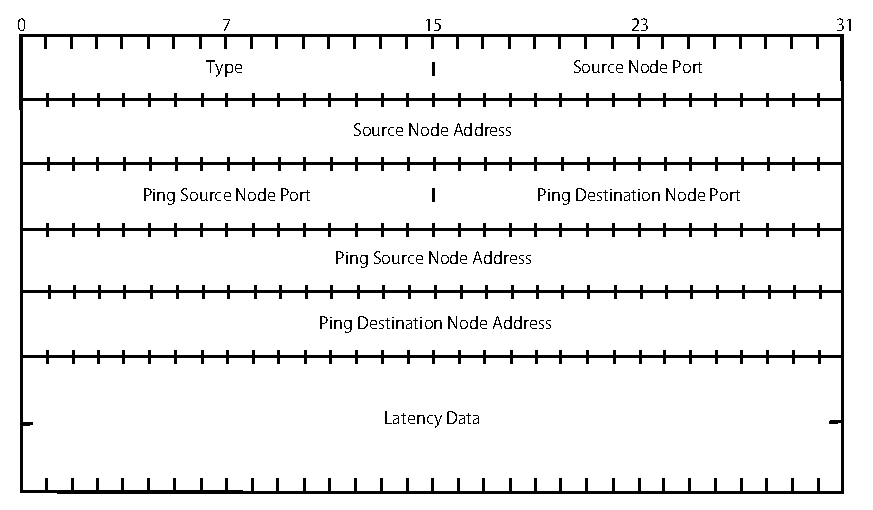
\includegraphics[scale=1.0]{./img/latencydatamessage}
		\caption{遅延データメッセージのフォーマット}
		\label{img:ldmessage}
	\end{center}
\end{figure}

\begin{figure}
	\begin{center}
		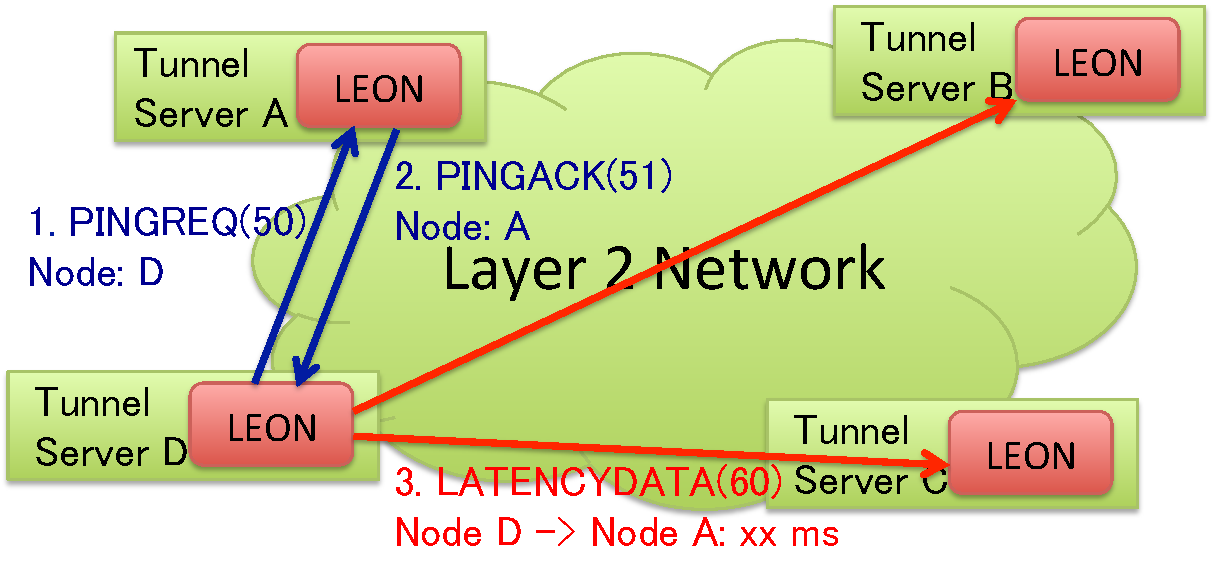
\includegraphics[scale=0.60]{./img/latencyproc}
		\caption{遅延データの共有プロセス}
		\label{img:ldproc}
	\end{center}
\end{figure}

トンネル終端点がトンネル終端点間の遅延を計測し、その計測結果を共有する際の手順を図~\ref{img:ldproc}
に示す。トンネル終端点間の遅延計測は定期的に全トンネル終端点で行われる。まず、トンネル終端点は
トンネル終端点が管理するトンネル終端点一覧に登録されている全トンネル終端点までの遅延を計測する。
遅延の計測を行うには、トンネル終端点は宛先のトンネル終端点に遅延計測メッセージを送信する。
遅延計測メッセージのTypeフィールドにはPINGREQ(50)、Source Node Addressフィールド、Node Addressフィールド
Source Node PortフィールドとNode Portフィールドには遅延計測を行うトンネル終端点のIPアドレスとポート番号を
挿入する。また、遅延計測を行うトンネル終端点は遅延計測メッセージの送信した時間を記憶する。そして、
遅延計測メッセージを受信したトンネル終端点は同様に遅延計測メッセージを返す。この時の遅延計測メッセージ
のTypeフィールドにはPINGACK(51)、Source Node Addressフィールド、Node Addressフィールド、Source Node Portフィールド
とNode Portフィールドには返信をするトンネル終端点のIPアドレスとポート番号を挿入する。遅延計測を行うトンネル終端点
が返信の遅延計測メッセージを受け取ると、受け取った時間から送信した時間の差から遅延を求める。そして、遅延を
遅延データベースに登録する。

また、トンネル終端点間の遅延計測結果は各トンネル終端点が経路選択を行う際に必要となる。そのため、
トンネル終端点は遅延計測結果を遅延データベースに登録後、遅延結果をトンネル終端点一覧に登録されて
いる全トンネル終端点に通知する。通知には遅延データメッセージが用いられる。遅延データメッセージには
遅延計測メッセージの送信元と送信先、及び、遅延の計測結果が含まれる。共通ヘッダー部分のTypeフィールド
にはLATENCYDATA(60)、Source Node AddressとSource Node Portフィールドには遅延データメッセージを送信
するトンネル終端点のIPアドレスとポート番号を挿入する。遅延データ部分のPing Source Node Addressフィールド
とPing Source Node Portフィールドには遅延計測メッセージを送信したトンネル終端点のIPアドレスとポート番号、
Ping Destination Node PortフィールドとPing Destination Node Addressフィールドには遅延計測メッセージを受信した
トンネル終端点のIPアドレスとポート番号、Latency Dataフィールドには遅延の計測結果を挿入する。この遅延データ
メッセージを受信したトンネル終端点は遅延データベースに指定されたトンネル終端点間の遅延データを登録する。
そして、収集された遅延データを用いて遅延が最も小さい経路を選択する。

\section{実装}
\label{solv:coding}

本節では、LEONの実装について述べる。本節では、本実装のことをleondと呼ぶ。

\subsection{実装環境}
\label{solv:codeenv}

表~\ref{table:codingenv}に本提案手法を実装するにあたり、利用した環境を示す。

\begin{table}[h]
	\begin{center}
		\caption{実装環境}
		\begin{tabular}{|l|l|}
			\hline
			CPU & Intel Xeon L5520 2.27Ghz * 2 (8 Cores) \\
			\hline
			RAM & 24GB DDR3 RAM \\
			\hline
			NIC & Intel 82575EB Gigabit NIC \\
			\hline
			使用OS & Debian 6.0.6 Squeeze \\
			\hline
			使用カーネル & Linux Kernel 3.7.2 \\
			\hline
			使用言語 & C言語 \\
			\hline
		\end{tabular}
		\label{table:codingenv}
	\end{center}
\end{table}

\subsection{実装概要}
\label{code:abst}

表~\ref{table:leonmods}にleondの各機構を構成するモジュールを示す。また、各モジュール間の関
係について図~\ref{img:leonoverview}に示す。

\begin{table}[h]
\begin{center}
	\caption{leondのモジュール}
	\begin{tabular}{|l|l|}
		\hline
		機構 & モジュール \\
		\hline
		\hline
		フレーム転送機構 & main\_poller \\
		終端点管理機構   & \\
		\hline
		遅延計測機構     & pinger \\
		\hline
		トポロジ構築機構 & topology \\
		\hline
		経路表 & fdb  \\
		       & nodelist \\
		\hline
	\end{tabular}
	\label{table:leonmods}
\end{center}
\end{table}

\begin{figure}
	\begin{center}
		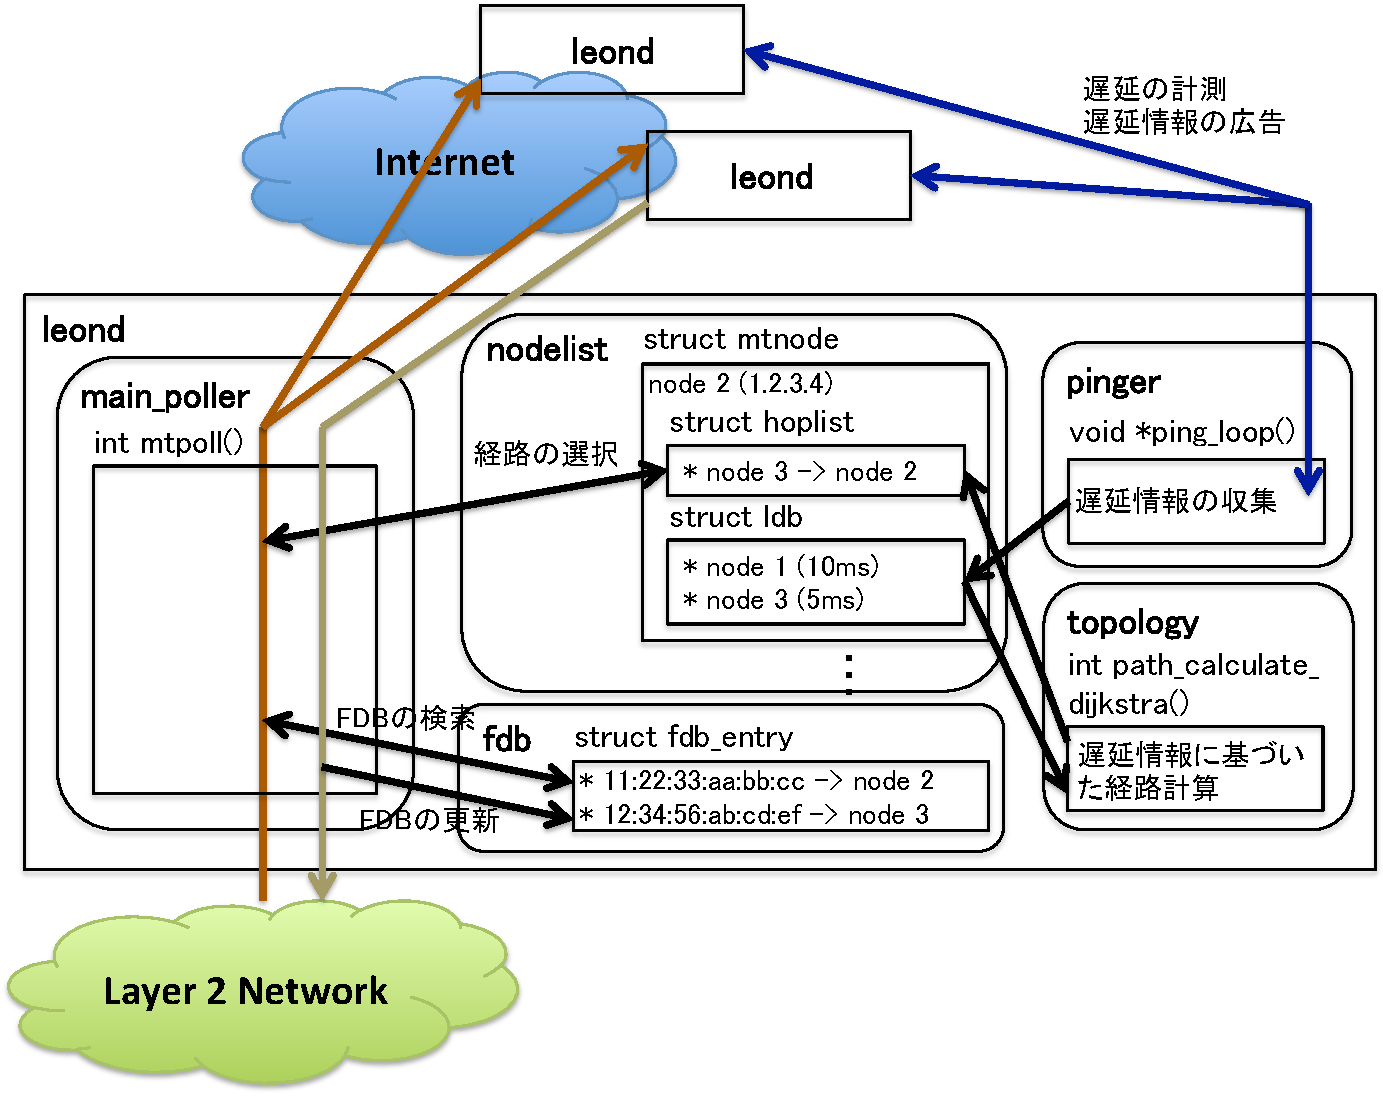
\includegraphics[scale=0.70]{./img/leonoverview}
		\caption{leondのモジュール間の関係}
		\label{img:leonoverview}
	\end{center}
\end{figure}

leondの引数と起動例を下記に示す。

\begin{verbatim}
$ ./leond
--debug: debug mode
-d: run as daemon
-u: localaddr:port
-p: peeraddr:port
--ping-interval: ping interval seconds

$ ./leond -d -u 1.2.3.4:10000 (既存のLayer 2ネットワークに参加しない場合)
$ ./leond -d -u 5.6.7.8:10000 -p 1.2.3.4:10000 (既存のLayer 2ネットワークに参加する場合)
\end{verbatim}

leondを起動するにあたり、必須である引数は\texttt{-u}オプションのみである。\texttt{-u}オプションには他のトンネル終端点からの
通信を待ち受けるために利用するIPアドレスとポート番号を指定する。また、既に他のトンネル終端点によって拡張
されているLayer 2ネットワークに参加する際には、既に参加しているトンネル終端点のIPアドレスとポート番号を
\texttt{-p}オプションで指定する。

また、遅延の計測を行う間隔のデフォルト値は60秒にした。デフォルト値から変更したい場合は、\texttt{--ping-interval}
オプションで遅延を計測する間隔を秒単位で指定することにより変更が可能である。デフォルト値を60秒に設定した理由は、
遅延の計測を小さい間隔で行うと、遅延データメッセージと遅延計測メッセージが大量に発生してしまう可能性があったからである。
Layer 2ネットワークに参加しているトンネル終端点の台数を$ N $、1回の遅延計測で発生するメッセージ数を$ M $とし、この2つの関係を数式で表すと次のようになる。

\begin{displaymath}
\displaystyle M = (2 + N) \times N
\end{displaymath}

そのため、例えば30台のトンネル終端点で、遅延計測の間隔を30秒とすると、30秒間で$ M = (2 + 30) \times 30 = 960 $個のメッセージが発生する。
この内、1台のトンネル終端点が処理するメッセージの量は$ 960 \div 30 = 32 $個である。32個のメッセージを30秒で処理するためには、トンネル終端点
は1秒に1個以上処理する必要がある。これではトンネル終端点が高負荷状態となり、イーサネットフレームの転送に遅延が発生する可能性があったので、
遅延計測の間隔を60秒とした。30台のトンネル終端点で、遅延計測の間隔が60秒の場合、トンネル終端点はメッセージを2秒に1個以上処理すれば良い。

\subsection{遅延計測機構}
\label{solv:latency}

遅延計測機構はpingerモジュールによって構成されている。pingerモジュールは、トポロジー構築機構に他トンネル終端点
にイーサネットフレームを転送するための経路を計算する際に必要となる情報を提供する。pingerモジュールの機能は3つある。
以下にそれぞれについて述べる。

まず1つ目のpingerモジュールの機能として、遅延データベースの管理が挙げられる。leondを利用して拡張されたLayer 2ネットワークに参加している
トンネル終端点の情報は、後述するnodelistモジュールが提供する\texttt{mtnode}構造体に記憶されている。\texttt{mtnode}構造体は参加している
トンネル終端点に対して1つ存在する。pingerモジュールは\texttt{mtnode}構造体の内部にある、\texttt{ldb}構造体の管理を行う。\texttt{ldb}構造体には
トンネル終端点間の遅延情報が記憶されている。pingerモジュールは遅延の計測結果、及び、他トンネル終端点から広告された
遅延情報を利用し\texttt{ldb}構造体の更新を行う。

2つ目のpingerモジュールの機能として他トンネル終端点までの遅延計測が挙げられる。遅延計測機能は起動時に\texttt{--ping-interval}オプションによって指定された時間毎
に呼び出される。起動時に指定されなかった場合は60秒毎に呼び出される。遅延計測機能が呼び出されると、~\ref{solv:latencyprotocol}項で説明した、
遅延計測メッセージを拡張されたLayer 2ネットワークに参加している全てのトンネル終端点に送信する。そして、他トンネル終端点から送信した遅延計測メッセージ
の返答を受け取ると、送信してから返信を受け取るまでに経過した時間を計算し、その時間を遅延として遅延データベースに登録する。また、遅延情報は
他のトンネル終端点が経路計算を同様に行うために必要となるため、全てのトンネル終端点に遅延情報を~\ref{solv:latencyprotocol}項で説明した、遅延データメッセージ
を用いて広告する。遅延データメッセージを受信したトンネル終端点は同様に、遅延情報を遅延データベースに登録する。

そして3つ目のpingerモジュールの機能として、トンネル終端点の死活監視が上げられる。
あるトンネル終端点から遅延計測メッセージの返信がない場合、そのトンネル終端点の遅延計測失敗回数を増加させる。失敗回数が2回になると、
そのトンネル終端点で障害が発生したと判断し、そのトンネル終端点をトンネル終端点リストから消去する。そして、トポロジー構築機構を呼び出し、
経路の再計算を行う。遅延計測失敗回数は、トンネル終端点から返信を受け取ると0に戻る。


\subsection{トポロジー構築機構}
\label{solv:dijkstra}

トポロジー構築機構はtopologyモジュールによって構成される。topologyモジュールは、leondを利用して拡張されたLayer 2ネットワークに参加している全てのトンネル終端点までの遅延が最も小さい
経路を計算する。フレーム転送機構はtopologyモジュールによって計算された経路を基に、イーサネットフレーム
の転送を行う。

topologyモジュールはpingerモジュールの遅延計測機能が呼び出された後に呼び出される。topologyモジュールが呼び出されると、
pingerモジュールによって収集された遅延データベースを基にダイクストラ法を用いて、トンネル終端点から拡張された
Layer 2ネットワークに参加している全てのトンネル終端点までの遅延が最も小さい経路の計算を行う。そして、
経路はフレーム転送機構が利用できるように、\texttt{mtnode}構造体の内部にある\texttt{hoplist}構造体に記憶する。topologyモジュールは
計算した経路を、経由するトンネル終端点の\texttt{mtnode}構造体へのポインターを、\texttt{hoplist}構造体に経由する順番通りにリスト構造状で
記憶する。

\subsection{経路表}
\label{solv:transfer}

経路表はfdbモジュールとnodelistモジュールによって構成される。nodelistモジュールは同一の拡張されたLayer 2ネットワークに参加している
トンネル終端点の情報を管理する。トンネル終端点の情報はnodelistモジュールが管理する\texttt{mtnode}構造体に格納される。\texttt{mtnode}構造体にはトンネル
終端点のIPアドレスとポート番号、遅延データベースである\texttt{ldb}構造体へのポインターとトンネル終端点へイーサネットフレームへ転送するための
経路情報が記憶されている\texttt{hoplist}構造体へのポインターが格納されている。他のモジュールがトンネル終端点の情報の追加や削除、検索を行う際には、
nodelistモジュールが提供するAPIを利用する。

また、fdbモジュールは拡張されたLayer 2ネットワーク内の各ホストがどのトンネル終端点によって収容されているかを学習する。fdbモジュールは
他のトンネル終端点から転送されたイーサネットフレームを受信した際に呼び出される。fdbモジュールが呼び出されると受信したイーサネットフレーム
の送信元ホストの\texttt{fdb\_entry}構造体が存在するか検索する。\texttt{fdb\_entry}構造体が存在しない場合は、新しい\texttt{fdb\_entry}構造体を作成し、その送信元ホスト
と転送したトンネル終端点の\texttt{mtnode}構造体へのポインターを記憶する。\texttt{fdb\_entry}構造体が存在する場合は、情報の更新が必要か確認し、必要の場合は更新
を行う。また、fdbモジュールは他のモジュールから\texttt{fdb\_entry}構造体の検索、更新、作成を行うためのAPIを提供する。フレーム転送機構がイーサネットフレーム
の転送を行う際には、fdbモジュールが提供するAPIを利用する。

\subsection{フレーム転送機構と終端点管理機構}
\label{solv:join}

フレーム転送機構と終端点管理機構はmain\_pollerモジュールによって構成されている。main\_pollerモジュールは他トンネル終端点
から受信した通信の処理、及び、トンネル終端点が収容しているホストから受信したイーサネットフレームの転送処理といった外部
からのイベント処理を行なっている。main\_pollerモジュールはLinuxのI/Oイベント通知機能であるepollを利用しイベントを待ち受ける。
そして、イベントが発生するとmail\_pollerモジュールの処理が開始する。

発生したイベントがトンネル終端点が収容しているホストからのイーサネットフレーム受信である場合、イーサネットフレームの転送処理
を行う。収容しているホストからイーサネットフレームを受信すると、イーサネットフレームの判別を行う。イーサネットフレームが
ブロードキャストフレームの場合は、全てのトンネル終端点に受信したイーサネットフレームを転送する。ユニキャストフレームの
場合は、送信先ホストをfdbモジュールが提供しているAPIを利用して検索し、転送先のトンネル終端点を決定する。そして、nodelist
モジュールが管理している\texttt{mtnode}構造体内の\texttt{hoplist}構造体に従って、~\ref{solv:fowardprotocol}項で説明した転送メッセージ
のパケットを生成する。最後に、生成した転送メッセージを\texttt{hoplist}構造体の一番最初に指定されているトンネル終端点へ転送する。

発生したイベントが他のトンネル終端点からの通信の場合、まず受信したメッセージの判別を行う。受信したメッセージが
転送メッセージの場合、転送メッセージの転送経路情報を確認する。受信した転送メッセージが自身宛の転送メッセージの場合は、
それを宛先ホストが収容されているLayer 2ネットワークへ転送する。それ以外の場合は、転送経路情報で指定されたトンネル終端点
へ転送メッセージを転送する。また、受信したメッセージがトンネル終端点の参加や離脱などを行うために利用されるコントロールメッセージの場合は、
nodelistモジュールが提供するAPIを利用し、nodelistモジュールの\texttt{mtnode}構造体を更新する。

%%% Local Variables:
%%% mode: japanese-latex
%%% TeX-master: "../yummy_bthesis"
%%% End:
